\section{App Komponenten}
\frame{
	\frametitle{Activities}
	TODO
}

% Bild einer (Sport-)Aktivität

\begin{frame}[c,fragile]
	\frametitle{Swing Button App}
	\begin{lstlisting}
	public static void main(String[] args) {
	    JFrame myFrame = new JFrame();
	    myFrame.addComponent(
	        new JButton("Click me!"));
	    myFrame.show();
	    ...
	}
	\end{lstlisting}
	\pause \vspace{0.5cm}
	\begin{figure}
	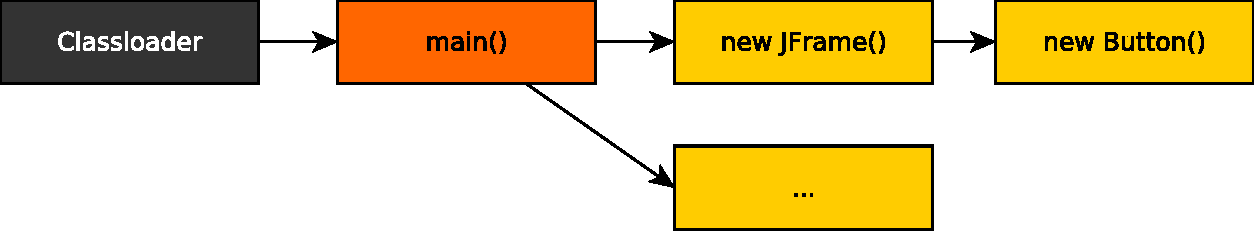
\includegraphics[width=\textwidth]{pictures/call-hierchy-swing.pdf}
	\end{figure}
\end{frame}

\frame[t]{
	\frametitle{Activities}
	% TODO Niko: Graphik MVC <-> Activity - Service - Content Provider + Intents + Broadcast Receiver
	\begin{itemize}
		\item View: Activity
		\item Controller: Service
		\item (Model: Content Provider)
		\item Kommunikation: Intents
		\item Listener: BroadcastReceiver
	\end{itemize}
}

\begin{frame}[c,fragile]
	\frametitle{Android Button App}
	\begin{lstlisting}[language=XML]
	<manifest>
	  <application label="ButtonApp">
	    <activity name=".MainActivity" 
	              label="Main Activity">
        ...
	</...>
	\end{lstlisting}
	\pause \vspace{0.5cm}
	\begin{lstlisting}
	class MainActivity extends Activity {
	    @Override
	    public void onCreate() {
	        //TODO add Button
	    }
	}
	\end{lstlisting}
\end{frame}

\frame[t]{
	\frametitle{Inversion of control}
	\centering
	\vspace{-0.2cm}
	\textbf{Swing}
	\begin{figure}
	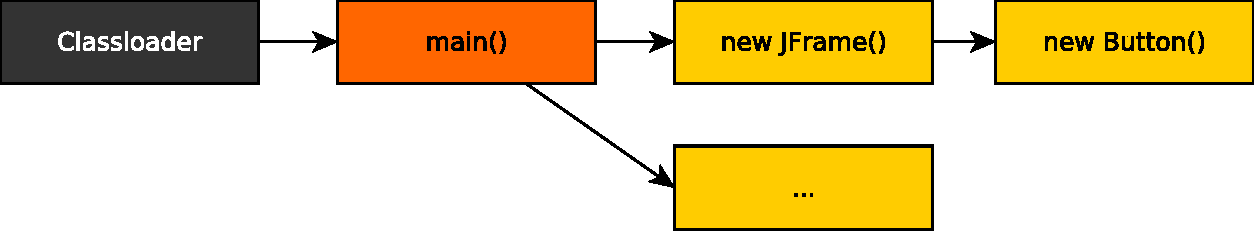
\includegraphics[width=0.8\textwidth]{pictures/call-hierchy-swing.pdf}
	\end{figure}
	\vspace{0.5cm}
	\textbf{Android}
	\begin{figure}
	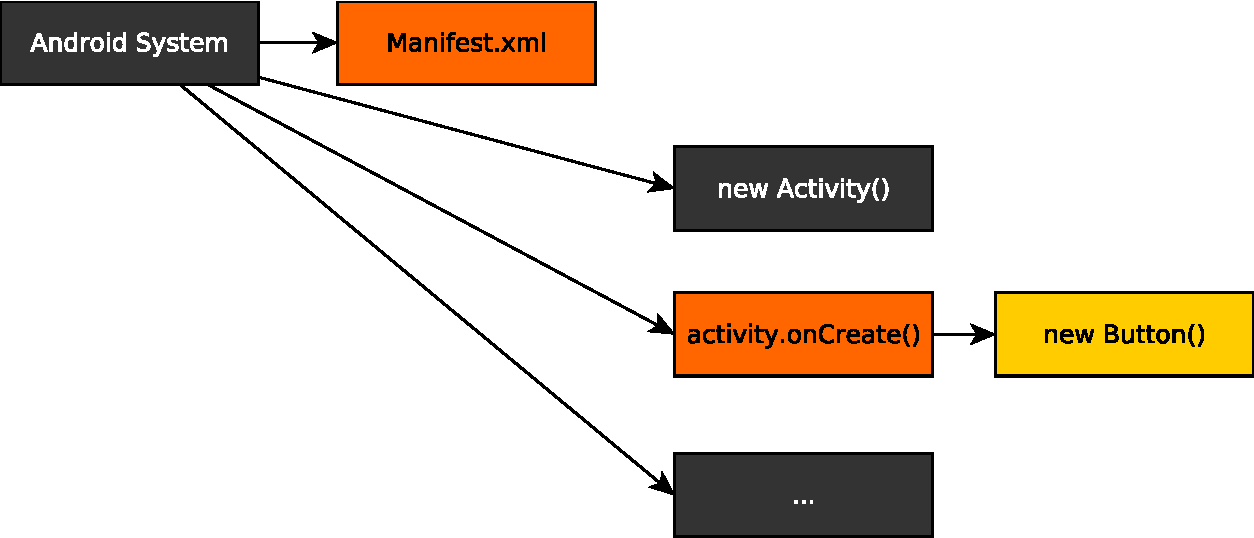
\includegraphics[width=0.8\textwidth]{pictures/call-hierchy-android.pdf}
	\end{figure}
}

\frame[c]{
	\frametitle{Activity Lifecycle}
	\begin{figure}
	\centering
	\includegraphics[width=\textwidth]{pictures/activity_lifecycle.png}
	\end{figure}
}

\frame[t]{
	\frametitle{Komponenten einer App}
	% TODO Niko: Graphik MVC <-> Activity - Service - Content Provider + Intents + Broadcast Receiver
	\begin{itemize}
		\item View: Activity
		\item Controller: Service
		\item (Model: Content Provider)
		\item Kommunikation: Intents
		\item Listener: BroadcastReceiver
	\end{itemize}
}

\frame[t]{
	\frametitle{Intents}
	% TODO Niko: intens als kommunikationsmittel in der App und zwischen apps
}